\documentclass[unicode,11pt,a4paper,oneside,numbers=endperiod,openany]{scrartcl}

\usepackage{amsmath, amssymb}
\usepackage{matlab-prettifier}
\usepackage{graphicx}
\usepackage{float}

\renewcommand{\thesubsection}{\arabic{subsection}}
\graphicspath{figures}

\input{assignment.sty}
\begin{document}


\setassignment
\setduedate{Wednesday, 6 December 2023, 11:59 PM}

\serieheader{Numerical Computing}{2023}{\textbf{Student:} Jeferson Morales Mariciano\\}
{\textbf{Discussed with:} Leonardo Birindelli, Michele Dalle Rive}
{Solution for Project 4}{}
\newline

\assignmentpolicy


\newpage

\section{General Questions [10 points]}

\subsection{What is the size of the matrix $A$?}
\label{ex:1.1}

In the context of Image Deblurring, where the problem defintion is
\begin{equation}\label{eq:problem}
    Ax = b
\end{equation}
matrix $A \in \mathbb{R}^{n^2 \times n^2}$ is the tranformation matrix
of an image of size $n \times n$ pixels, resulting from application of image kernel.\\
Given the original image matrix $X \in \mathbb{R}^{n \times n}$,
It is then vectorized to $x \in \mathbb{R}^{n^2}$,
where entries of $X$ are stacked either row or column wise.\\
The blurred image is $B \in \mathbb{R}^{n \times n}$,
and its vectorized form is denoted as $b \in \mathbb{R}^{n^2}$.\\\newline
Matrix $A$ can be very large as its growth is exponential to the image size,
thus is important to use sparse data structures.\\
In particular, the matrix in \textit{blur\_data/A.mat} path is defined as:
$A \in \mathbb{R}^{62500 \times 62500}$,
where $n = 250$ visibly resulting from blured image $B \in \mathbb{R}^{250 \times 250}$
from \textit{blur\_data/B.mat}.

\begin{lstlisting}[
        frame=single,
        numbers=left,
        style=Matlab-editor,
        basicstyle=\mlttfamily\small,
        label={lst:ex1-1},
        caption={script to calculate size of matrix A},
        captionpos=b]
load('blur_data/A.mat');
size(A)
\end{lstlisting}

\subsection{How many diagonal bands does $A$ have?}
Transformation matrix $A$ is $d^2$-banded with $d \ll n$, hence $d \ll 250$.\\
The blurred image pixel is the weighted average of the surrounding pixels,
such weights are defined by the kernel
matrix $K \in \mathbb{R}^{d \times d}$.
The bigger transformation matrix $A$ is constructed from the kernel matrix,
such that the non-zero elements of each row of $A$ correspond to the values of $K$.\\
\[
    K =
    \frac{1}{605}
    \begin{bmatrix}
        100 & 9 & 9 & 9 & 9 & 9 & 100 \\
        9   & 1 & 1 & 1 & 1 & 1 & 9   \\
        9   & 1 & 1 & 1 & 1 & 1 & 9   \\
        9   & 1 & 1 & 1 & 1 & 1 & 9   \\
        9   & 1 & 1 & 1 & 1 & 1 & 9   \\
        9   & 1 & 1 & 1 & 1 & 1 & 9   \\
        100 & 9 & 9 & 9 & 9 & 9 & 100 \\
    \end{bmatrix}
    \in \mathbb{R}^{7 \times 7}
\]

Hence, $A$ has $d^2 = 7^2 = 49$ diagonal bands.

\subsection{What is the length of the vectorized blurred image $b$?}

From Exercise \ref{ex:1.1}, problem defintion equation \ref{eq:problem},
the length of vectorized blurred image $b$ is $n^2$.\\
Remember that the vectorization order for this assignment is row-wise,
though Matlab default is column-wise.\\
The length of $b$ is $62500$.

\begin{lstlisting}[
        frame=single,
        numbers=left,
        style=Matlab-editor,
        basicstyle=\mlttfamily\small,
        label={lst:ex1-3},
        caption={script to calculate length of vectorized blurred image $b$},
        captionpos=b]
B = B';
b = B(:);
length(b)  
\end{lstlisting}

\section{Properties of A [10 points]}

\subsection{If $A$ is not symmetric, how would this affect $\tilde{A}$?}

To use the conjugate gradient method, the matrix $A$ must be symmetric positive-definite.\\
Even if initially $A$ is not symmetric, after solving the augmented equation:
\[
    \underbrace{A^\intercal A}_{\tilde{A}} x = \underbrace{A^\intercal b}_{\tilde{b}}
\]
$\tilde{A}$ will be symmetric since the product of any matrix and its transpose
always produces a symmetric matrix.\\

\subsection{Explain why solving $Ax = b$ for $x$ is equivalent to minimizing
    $\frac{1}{2}x^\intercal Ax - b^\intercal x$ over $x$,
    assuming that $A$ is symmetric positive-definite.}

Instead of solving $Ax = b$,
assume precondition:
matrix $A$ is symmetric and positive definite (SPD), meaning
\[ \langle Ax, x \rangle > 0 \text{, if } x \neq \underline{0} \]
Then, solve the minimization problem:
\[ f(x) := \frac{1}{2} \langle Ax, x \rangle - \langle b, x \rangle \]
Now, let's find the derivative of $f(x)$ with respect to $x$.
\begin{align*}
    f(x) & = \frac{1}{2} \langle Ax, x \rangle - \langle b, x \rangle \\
         & = \frac{1}{2} x^T A x - b^T x
\end{align*}

The derivative of the quadratic form $x^T A x$ with respect to $x$ is given by
\[ \frac{d}{dx}(x^T A x) = (A + A^T)x \]

Therefore, the derivative of $f(x)$ with respect to $x$ is
\begin{align*}
    \frac{df}{dx} & = \frac{1}{2} \frac{d}{dx}(x^T A x) - \frac{d}{dx}(b^T x) \\
                  & = \frac{1}{2} (A + A^T)x - b
\end{align*}

So, the result is
\[ \frac{df}{dx} = \frac{1}{2} (A + A^T)x - b \]

Remember, since matrix $A$ is symmetric, then $A^\intercal = A$, thus:
\begin{align*}
     & = \frac{1}{2} (A + A^\intercal)x - b \\
     & = \frac{1}{2} (A + A)x - b           \\
     & = Ax - b
\end{align*}

Finally, it becomes clear why solving $Ax = b$ is equivalent to minimizing
$\frac{1}{2} x^\intercal A x - b^\intercal x$ over $x$ with assumptions on $A$ being SPD.


\section{Conjugate Gradient [30 points]}

\subsection{Write a function for the conjugate gradient solver
        [x,rvec]=myCG(A,b,x0,max itr,tol),
    where x and rvec are, respectively, the solution value and a vector
    containing the residual at every iteration.}

The file containing the solution can be found in \textit{myCG.m} matlab script file.

\subsection{In order to validate your implementation,
    solve the system defined by A\_test.mat and b\_test.mat.
    Plot the convergence (residual vs iteration).}

Hereby, it is shown the relation between residual and iterations during convergence
in both bar chart in Figure \ref{fig:ex3-2-bar} and logarithmic chart in Figure \ref{fig:ex3-2}.

\begin{figure}[H]
    \centering
    \caption{Convergence, residual vs iteration}
    \label{fig:ex3-2-bar}
    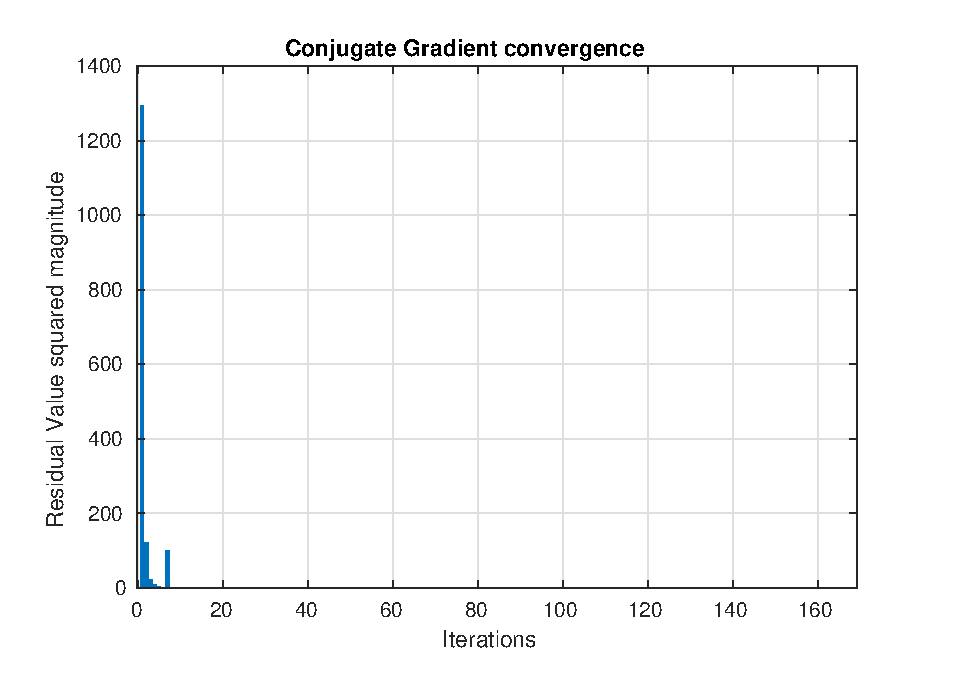
\includegraphics[width=\textwidth, trim={0cm 0cm 0cm 0cm}]{./figures/ex3-2-bar.eps}
\end{figure}

\begin{figure}[H]
    \centering
    \caption{Convergence, residual vs iteration - logarithmic view}
    \label{fig:ex3-2}
    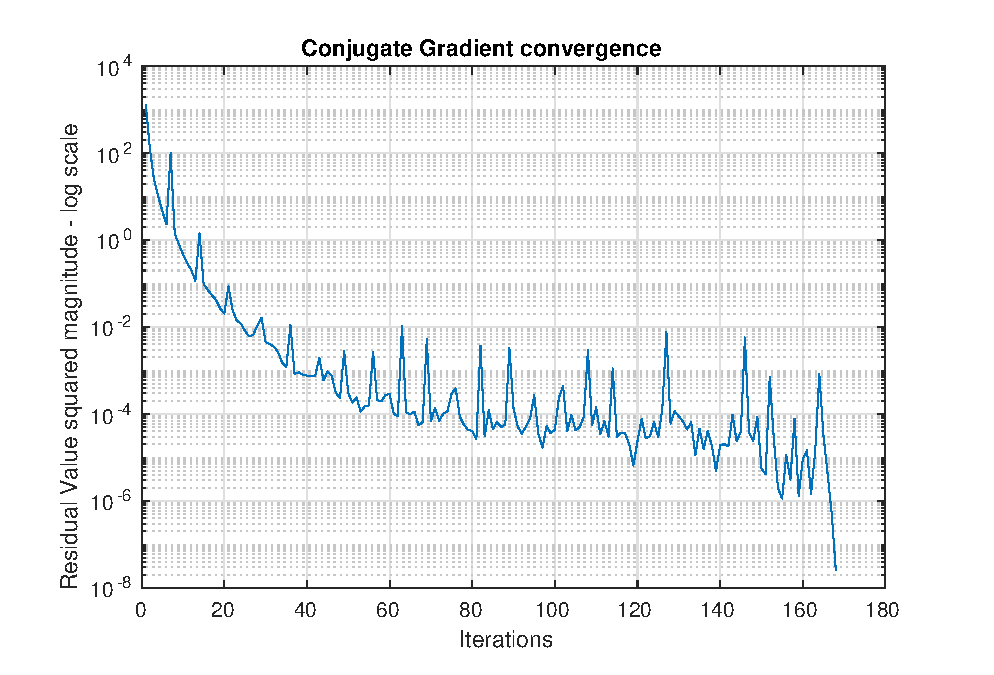
\includegraphics[width=\textwidth, trim={0cm 0cm 0cm 0cm}]{./figures/ex3-2.eps}
\end{figure}

\subsection{Plot the eigenvalues of A\_test.mat
    and comment on the condition number and convergence rate.}

The eigenvalues of matrix $A$ are plotted in Figure \ref{fig:ex3-3}.\\
Recall that condition number of a matrix is defined as the ratio of the largest
to the smallest singular value, and if very big, it indicates the matrix is ill-conditioned. \\
\[k(A) = \frac{\sigma_{max}}{\sigma_{min}}\]
where $\sigma$ indicates singular values of $A$.\\
The condition number of $A_{test}$ at start is computed with matlab
with the \textit{cond($A_{test}$)} command.\\
The results is $k(A) = 1.3700e+06 = 1.37 * 10^6$, a huge number explaining why that convergence
of the Conjugate Gradient method is slow paced since the convergence is hinderend with such a high number.

\begin{figure}[H]
    \centering
    \caption{Eingenvalues of matrix A}
    \label{fig:ex3-3}
    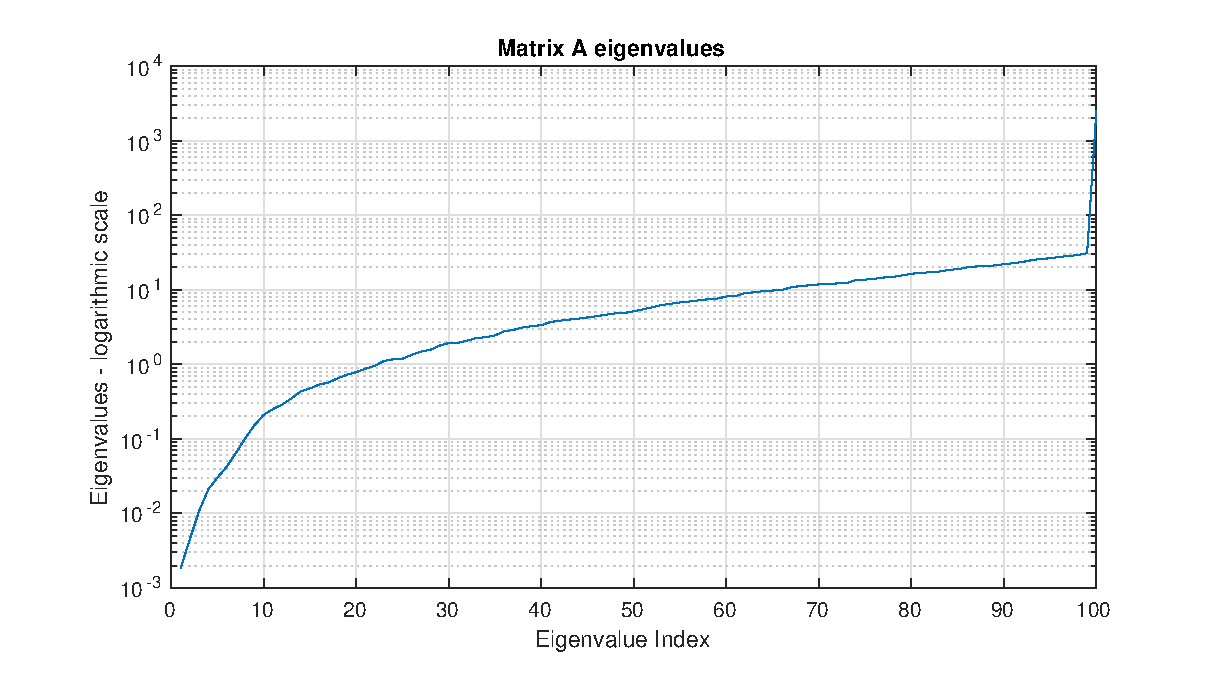
\includegraphics[width=\textwidth, trim={0cm 0cm 0cm 0cm}, clip]{./figures/ex3-3.eps}
\end{figure}

\subsection{Does the residual decrease monotonically? Why or why not?}

Figures \ref{fig:ex3-2-bar}, \ref{fig:ex3-2} strongly suggest the residuals are not monotonically decreasing
by presenting peaks along the chart,
despite the Conjugate Gradient method supposed to monotonically improving approximations of $x_k$
to the exact solution.
The relation with the CG method is explainable because of its inner instability
with respect to small pertubations, particularly considering the fact that its speed is determined
by the condition number $k(A)$ of the system matrix, meaning: the larger $k(A)$, the slower the improvement.\\

Apporting small perturbations to decrease the condition number, e.g. preconditioning,
should denote approximations of $x_k$ being monotonically more accurate during the iterative method.

\section{Deblurring problem [35 points]}

\subsection{Solve the deblurring problem for the blurred image matrix B.mat
    and transformation matrix A.mat using your routine myCG and Matlab's preconditioned conjugate gradient pcg.
    As a preconditioner, use ichol to get the incomplete Cholesky factors and set routine type to nofill
    with $\alpha = 0.01$ for the diagonal shift (see Matlab documentation).
    Solve the system with both solvers using $max\_iter = 200$, $tol = 10^{-6}$.
    Plot the convergence (residual vs iteration) of each solver and display the original and final deblurred image.
    Comment on the results that you observe.}

Figure \ref{fig:ex4-1-blurred}, \ref{fig:ex4-3-deblurred-cg} show respectively the blurred image
and the deblurred one using the assignment own implementation of Conjugate Gradient method.\\
The plot in Figure \ref{fig:ex4-4-residual-cg} show the relation of the residual squared magnitude using the
Conjugate Gradient method.\\

Figure \ref{fig:ex4-5-blurred}, \ref{fig:ex4-6-pcg} show respectively the blurred image
and the deblurred one using the Preconditioned Conjugate Gradient method.\\
Such method uses the incomplete Cholesky factorization as preconditioner, already implemented in matlab API
with function signatures \textit{ichol(...)}.
The plot in Figure \ref{ex4-7-residual-pcg} show the relation of the residual squared magnitude using the
Preconditioned Conjugate Gradient method.\\

The precondiotioned method converge way faster as it is visible from the plots.
Such phenomenon is due to the fact that the condition number, computed with
$condest(\tilde{A}) = 2.0501e+11 = 2.0501 * 10^{11}$
is very high and thus the preconditioner method is capable to show off its potential by reducing
the condition number and reach convergence in a very smaller number of iterations than simple
Conjugate Gradient Method.

\begin{figure}[H]
    \centering
    \caption{Blurred Image}
    \label{fig:ex4-1-blurred}
    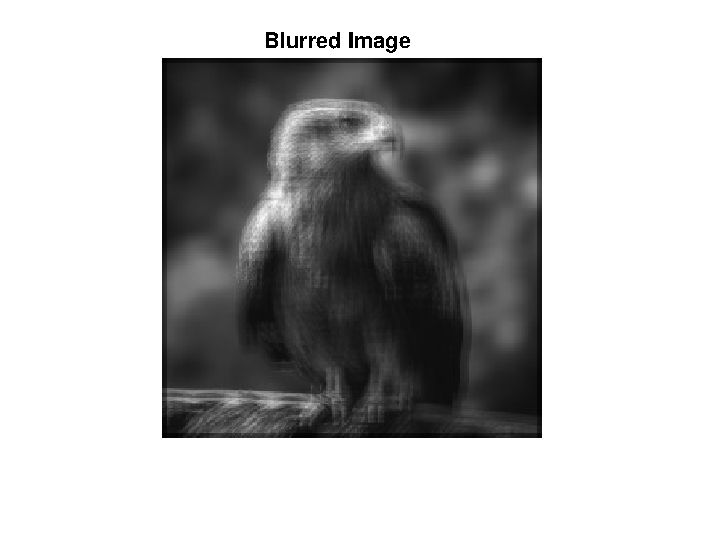
\includegraphics[width=\textwidth, trim={0cm 0cm 0cm 0cm}, clip]{./figures/ex4-1-blurred.eps}
\end{figure}

\begin{figure}[H]
    \centering
    \caption{Deblurred Image using CG method}
    \label{fig:ex4-3-deblurred-cg}
    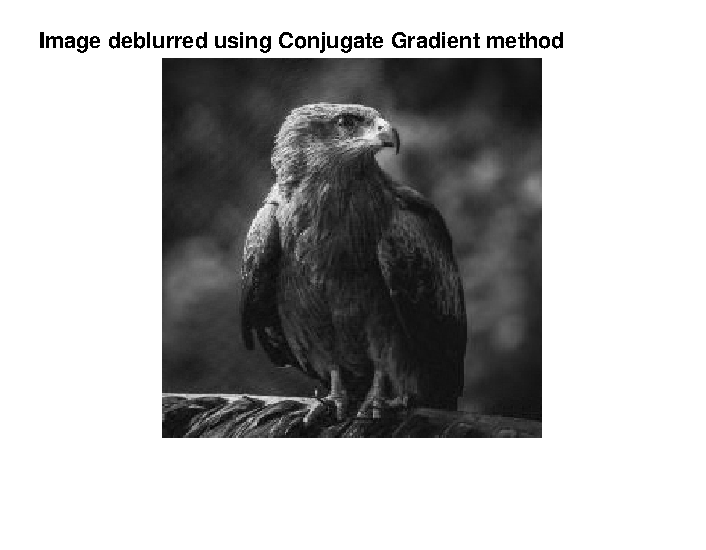
\includegraphics[width=\textwidth, trim={0cm 0cm 0cm 0cm}, clip]{./figures/ex4-3-deblurred-cg.eps}
\end{figure}

\begin{figure}[H]
    \centering
    \caption{Relation between residual squared magnitude and iterations with CG method}
    \label{fig:ex4-4-residual-cg}
    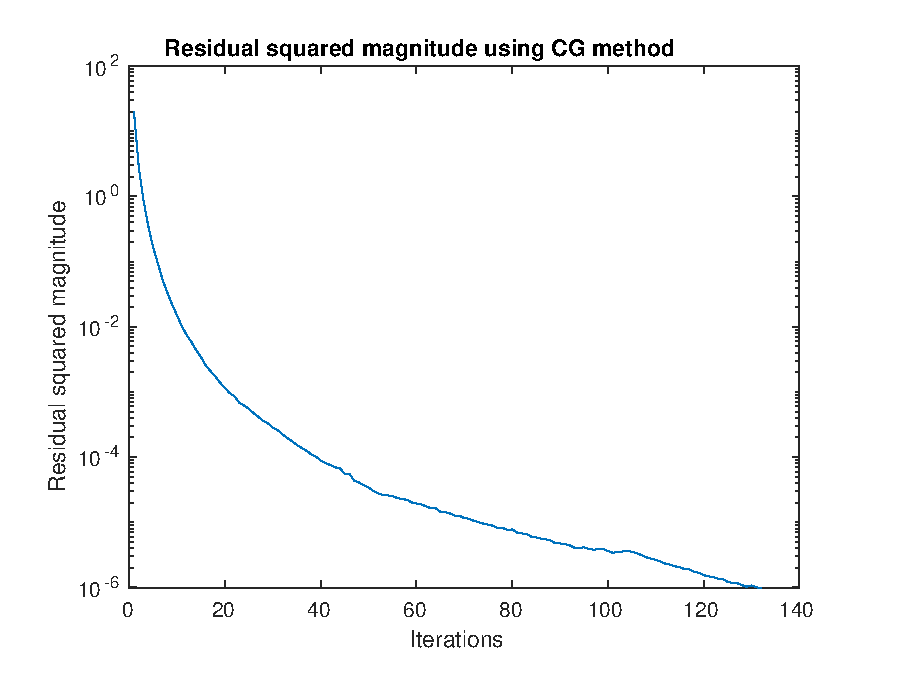
\includegraphics[width=\textwidth, trim={0cm 0cm 0cm 0cm}, clip]{./figures/ex4-4-residual-cg.eps}
\end{figure}


\begin{figure}[H]
    \centering
    \caption{Blurred Image}
    \label{fig:ex4-5-blurred}
    \includegraphics[width=\textwidth, trim={0cm 0cm 0cm 0cm}, clip]{./figures/ex4-5-blurred.eps}
\end{figure}

\begin{figure}[H]
    \centering
    \caption{Deblurred Image using PCG preconditioning}
    \label{fig:ex4-6-pcg}
    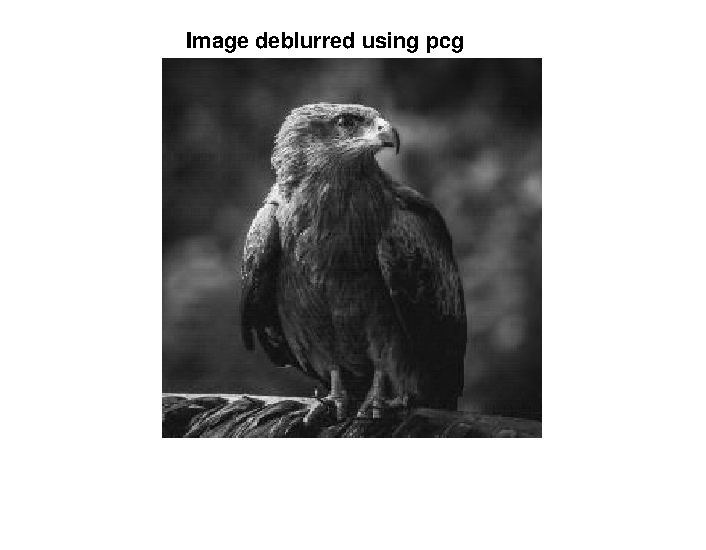
\includegraphics[width=\textwidth, trim={0cm 0cm 0cm 0cm}, clip]{./figures/ex4-6-pcg.eps}
\end{figure}

\begin{figure}[H]
    \centering
    \caption{Relation between residual squared magnitude and iterations with PCG preconditioning}
    \label{fig:ex4-7-residuals-pcg}
    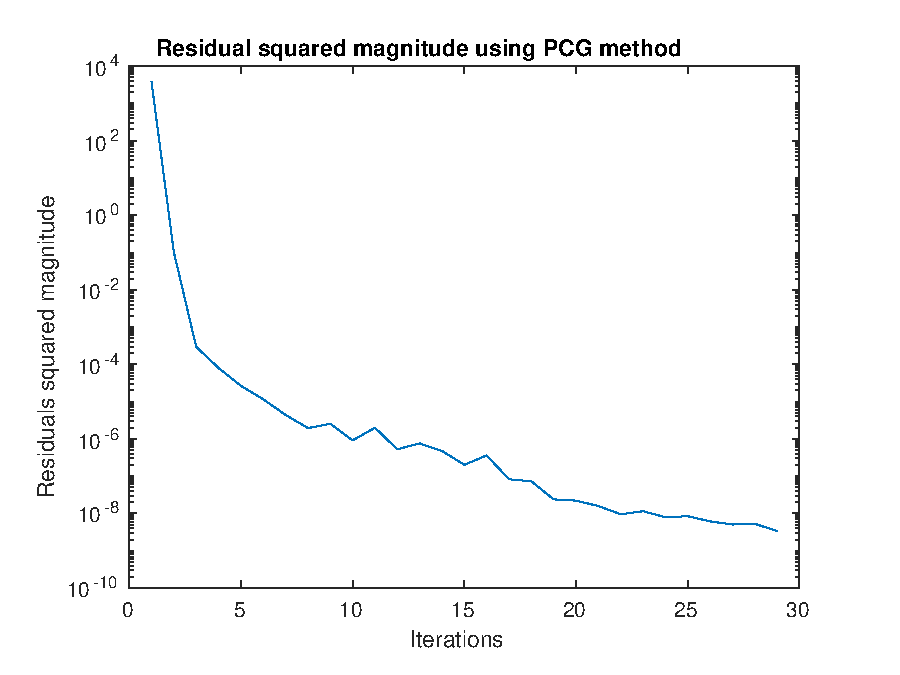
\includegraphics[width=\textwidth, trim={0cm 0cm 0cm 0cm}, clip]{./figures/ex4-7-residuals-pcg.eps}
\end{figure}

\subsection{When would pcg be worth the added computational cost? What about if you are deblurring lots of images with
    the same blur operator?}

The preconditioning must be stored in memory and for very large matrix it cannot be feasible.\\
Such method have indeed strong advantages but when the memory size is impractical are even impossible to
reach if it is in the magnitude of Terabytes, then is discorauged.\\
Keep in mind that if the condition number is indeed extremely large, such method even for large
matrices can be taken into consideration.\\
Moreover, the computational cost of the preconditioning could be distributed into multiple systems
to increase feasibility, and can be a great advantages if the matrix is reused multiple times
since it is enough to compute it once.

\end{document}
